\begin{frame}
    \frametitle{Completed Stage 2-2: ROLLO v1.0 Demonstration}
    \begin{itemize}
        \item Single objective design problem: maximize $k_{eff}$ by varying 
        TRISO particle distribution in an AHTR fuel slab while keeping total 
        packing fraction constant
        \item A sine distribution governs the TRISO particle packing fraction's 
        distribution across 10 cells:
    \end{itemize}
    \begin{align*}
        PF(x) &= \left(a\cdot sin(b\cdot x + c) + 2\right) \cdot NF
    \end{align*}
    \begin{figure}[]
        \centering
        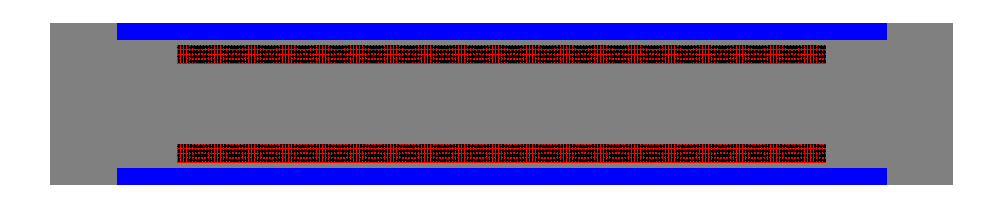
\includegraphics[width=0.6\linewidth]{../docs/figures/straightened_slab.png} 
    \end{figure}
    \begin{figure}[]
        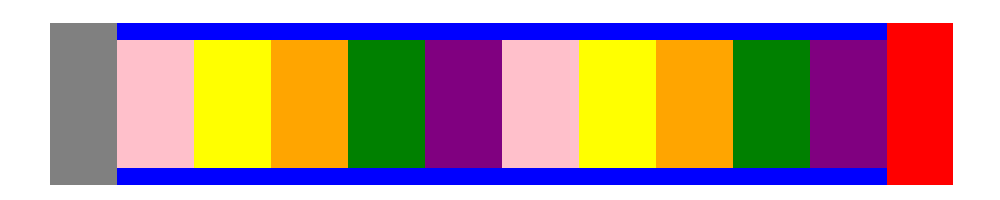
\includegraphics[width=0.6\linewidth]{../docs/figures/straightened_slab_mg.png}
        \caption{AHTR fuel slab spatially discretized into 13 cells with varying 
        TRISO particle distributions in 10 cells.}
    \end{figure}
\end{frame}

\begin{frame}
    \frametitle{Completed Stage 2-2: Problem Definition}
    \begin{figure}[]
        \centering
        \makebox[\textwidth][c]{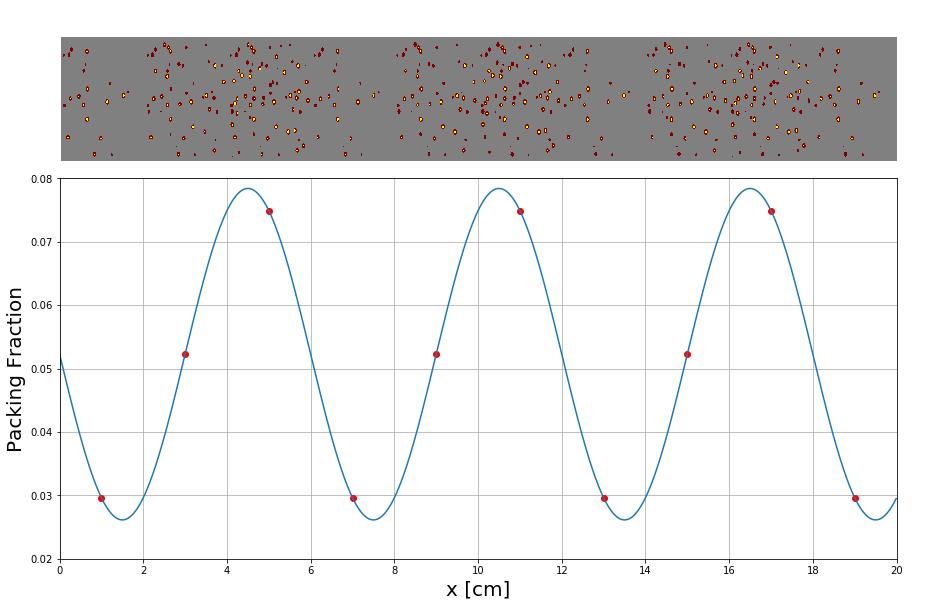
\includegraphics[width=0.9\linewidth]{../docs/figures/triso_distribution_sine.png}} 
        \caption{Above: AHTR fuel slab with varying TRISO particle 
        distribution across ten cells based on the sine distribution. 
        Below: $PF(x) = (0.5\ sin(\frac{\pi}{3}x + \pi) + 2)  \times NF$ 
        sine distribution with red points indicating the packing fraction at each cell.}
    \end{figure}
\end{frame}

\begin{frame}
    \frametitle{Completed Stage 2-2: Problem Definition}
    \begin{minipage}[c]{0.6\textwidth}
    \begin{figure}
        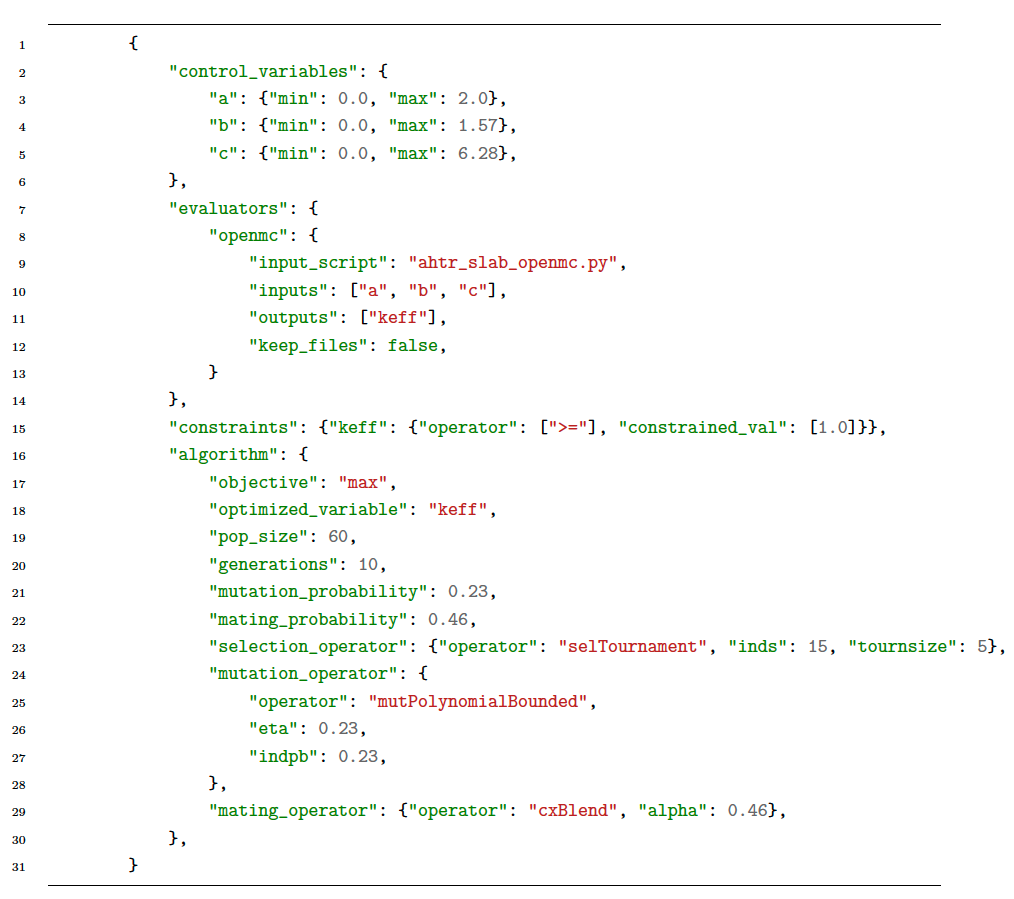
\includegraphics[width=0.9\linewidth]{figures/ii2-rollo-input.png}
        \caption{ROLLO JSON input file.}
    \end{figure}
\end{minipage}\hfill
    \begin{minipage}[c]{0.4\textwidth}
        \centering
        \begin{figure}
            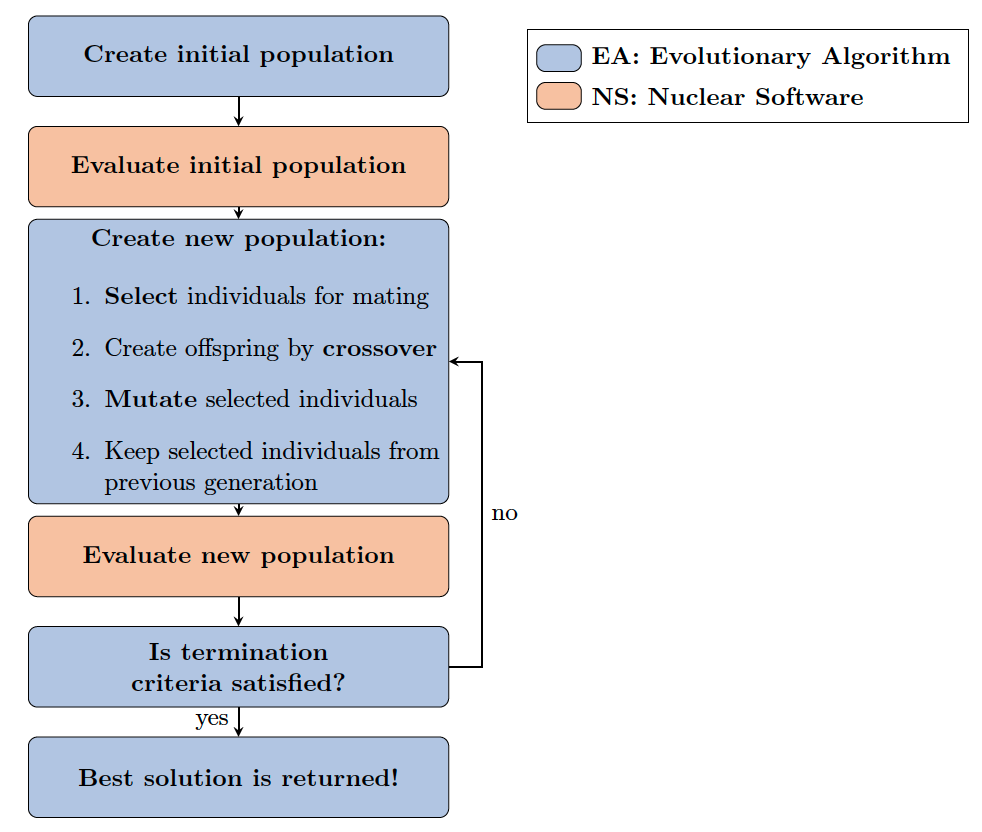
\includegraphics[width=\linewidth]{figures/rollo-flow.png} 
            \caption{ROLLO's flow.}
        \end{figure}
    \end{minipage}
    \scriptsize
    OpenMC runs each simulation with 80 active cycles, 20 inactive cycles, and 
    8000 particles to reach $\sim$130pcm uncertainty.
\end{frame}

\begin{frame}
    \frametitle{Completed Stage 2-2: Hyperparameter Search}
    \begin{itemize}
        \item A good hyperparameter set guides the optimization process by 
        balancing exploitation and exploration to find an optimal solution quickly 
        and accurately
        \item I performed the hyperparameter search with a coarse-to-fine random 
        sampling scheme
    \end{itemize}
    \begin{figure}[]
        \centering
        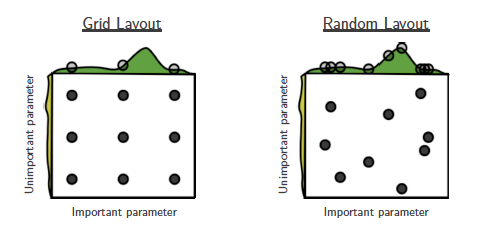
\includegraphics[width=0.5\linewidth]{../docs/figures/random_vs_grid_sampling.png} 
        \caption{The impact of grid sampling vs random sampling on coverage of projections 
        into subspaces (reproduced from \cite{jordan_hyperparameter_2017}). 
        Random sampling has better coverage in the subspaces.}
    \end{figure}
\end{frame}

\begin{frame}
    \frametitle{Completed Stage 2-2: Hyperparameter Search}
    \begin{itemize}
        \item I started with 25 coarse experiments and fine-tuned the hyperparameters
        with 15 more experiments
        \item For each genetic algorithm experiment, the number 
        of OpenMC evaluations remained constant at 600
    \end{itemize}
    \begin{table}
        \caption{Hyperparameter search is conducted in three phases: \textit{Coarse Search}, 
    \textit{Fine Search 1}, \textit{Fine Search 2}. Each hyperparameter's lower and
    upper bounds for each search phase are listed.}
        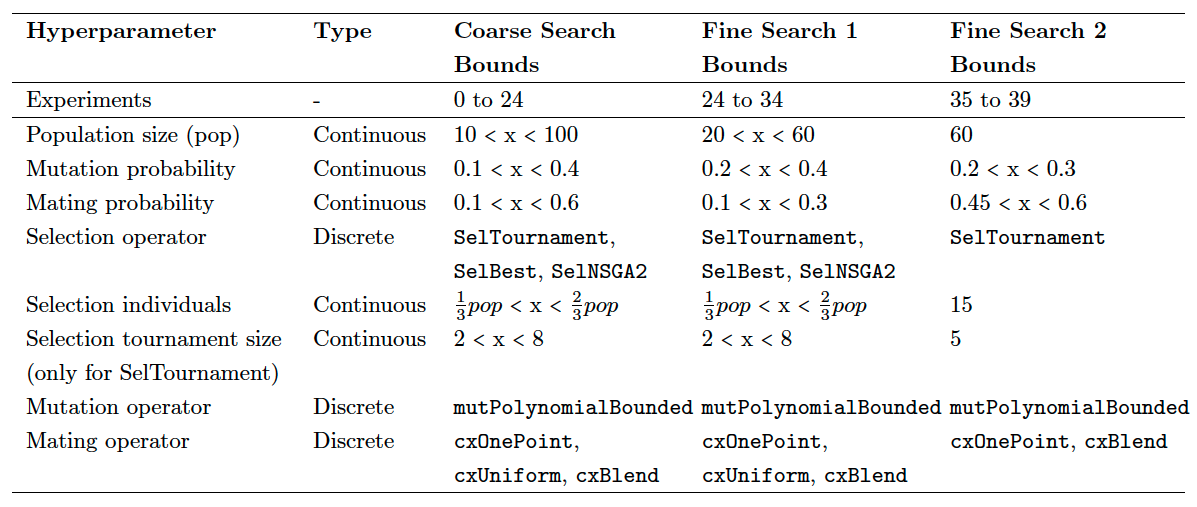
\includegraphics[width=0.8\linewidth]{figures/hyperparameter-search.png} 
    \end{table}
\end{frame}

%\begin{frame}
%    \frametitle{Completed Stage 2-2: Hyperparameter Search}
%    \begin{figure}[]
%        \centering
%        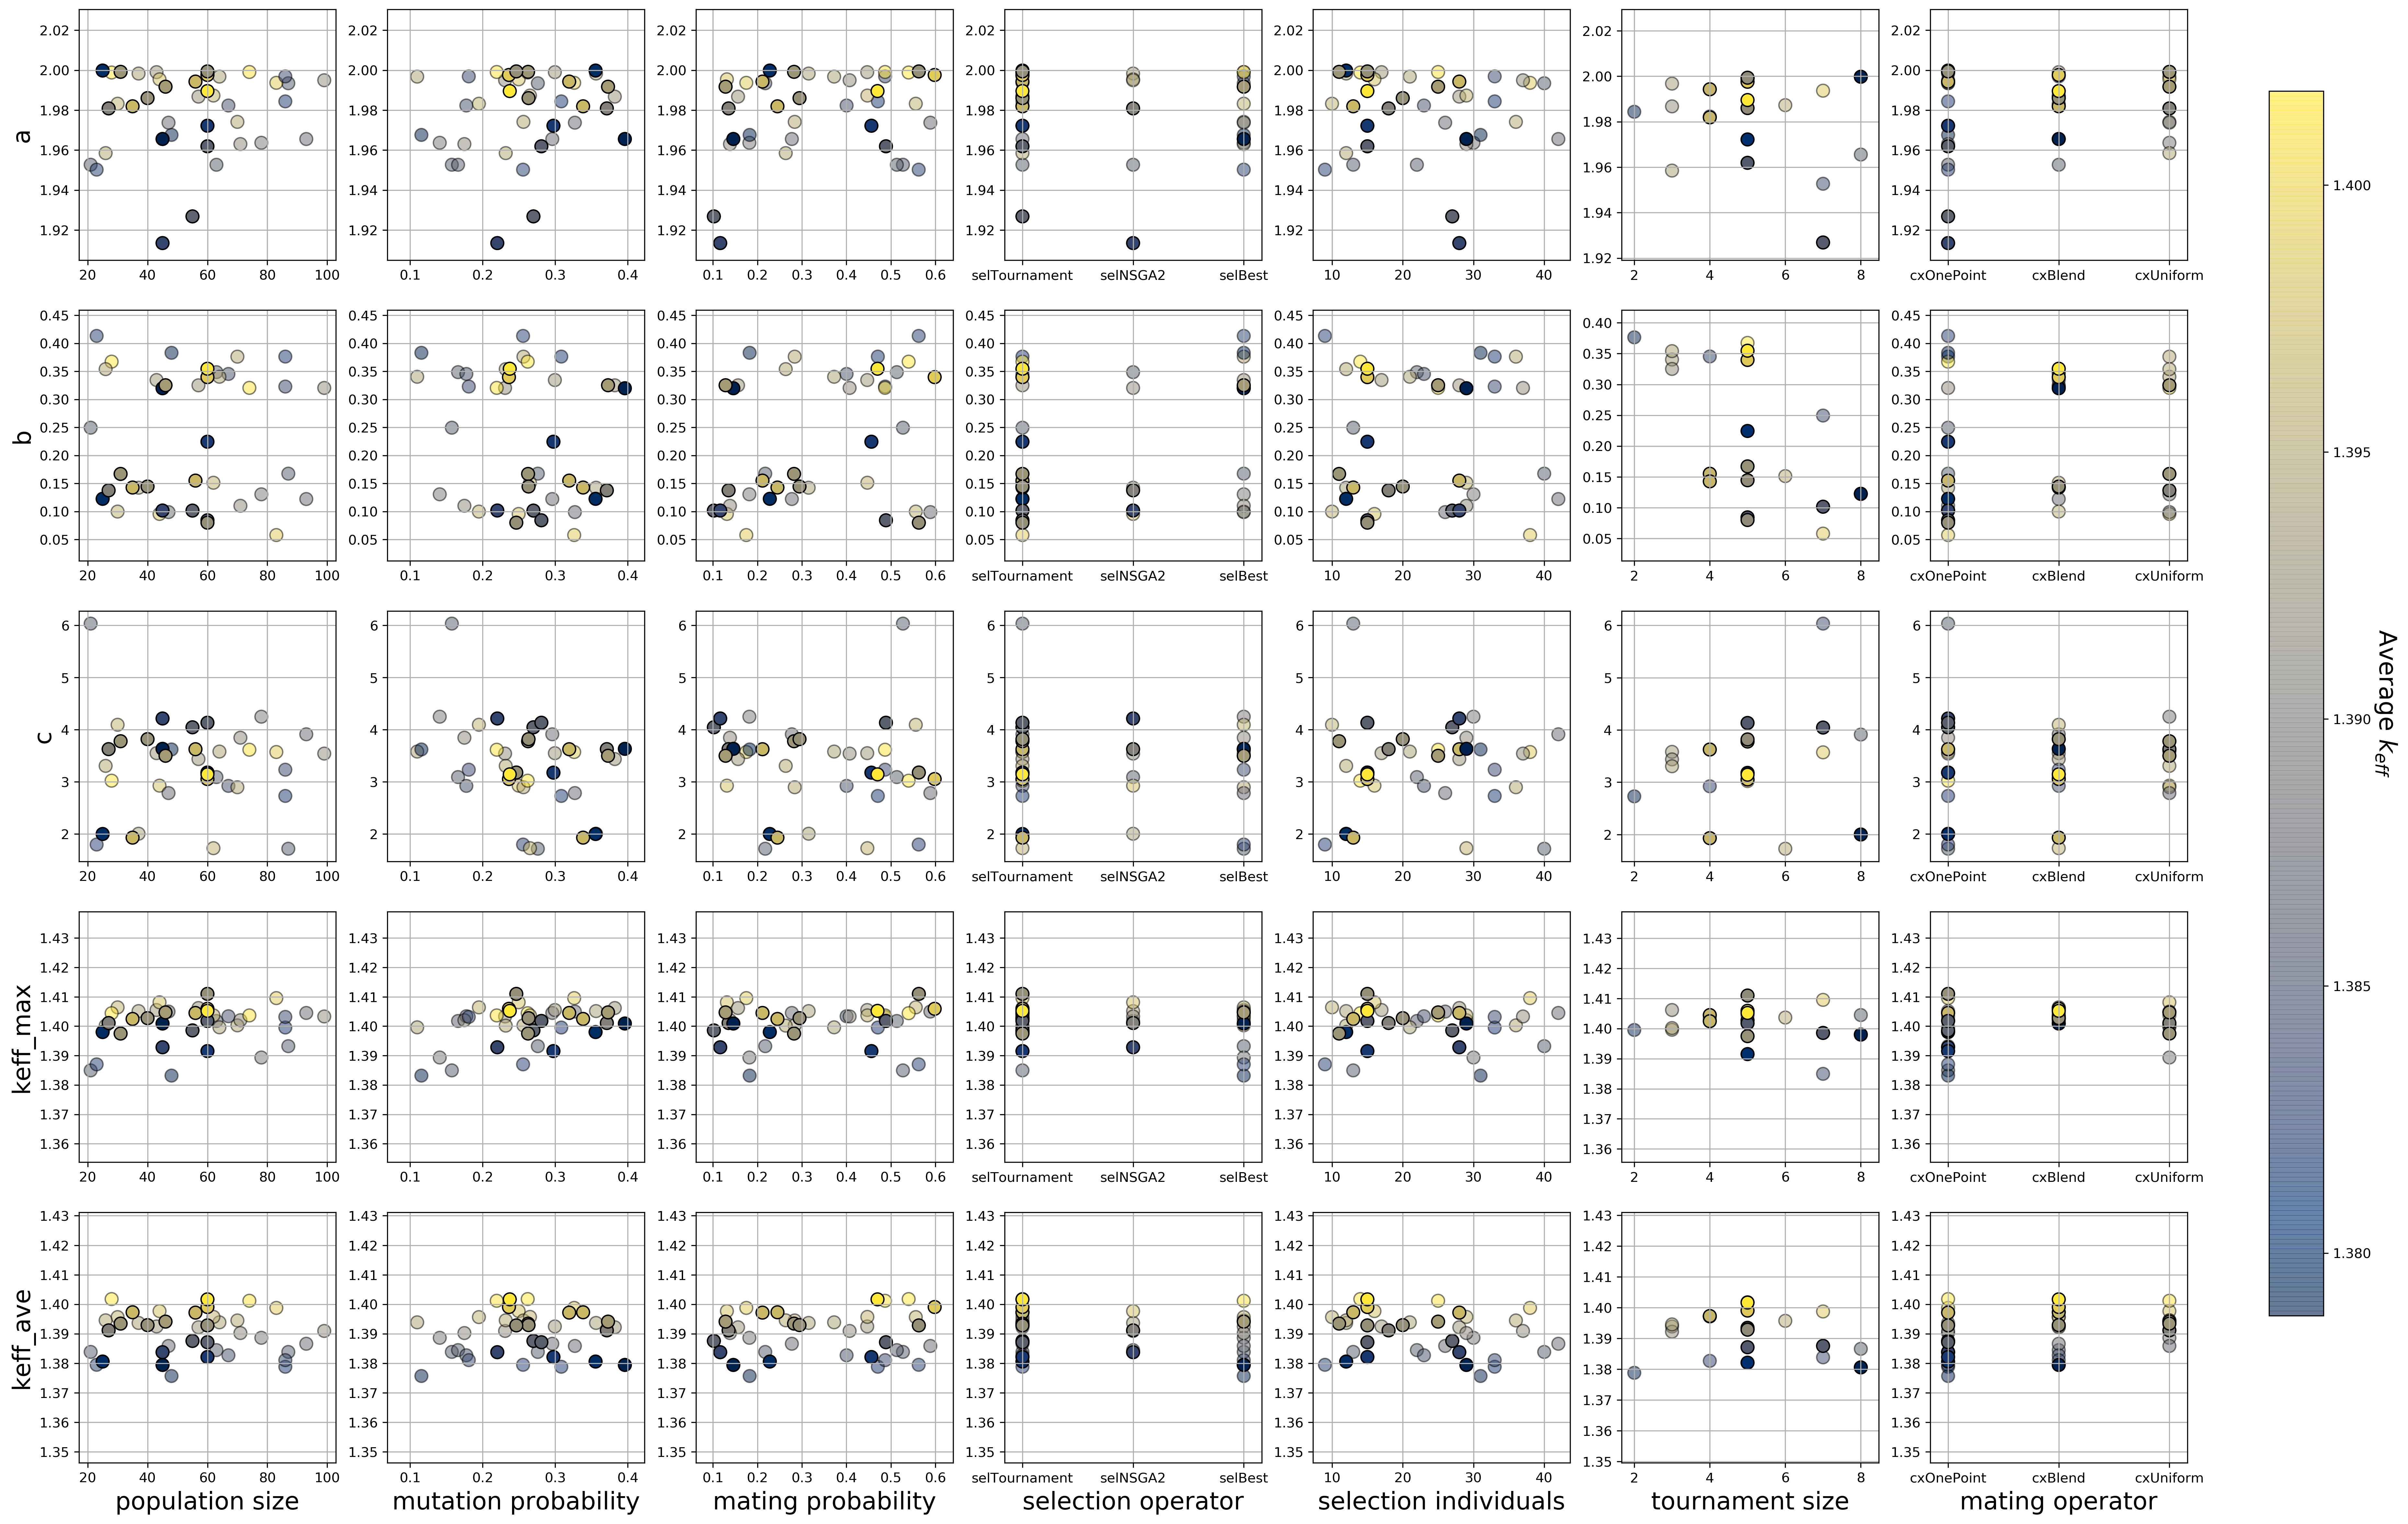
\includegraphics[width=0.85\linewidth]{../docs/figures/input_hyperparameters_sens.png} 
%        \caption{Hyperparameters search's results for all 40 experiments (coarse 
%        and fine).}
%    \end{figure}
%\end{frame}

\begin{frame}
    \frametitle{Completed Stage 2-2: Results from best hyperparameter set}
    \begin{table}
        \caption{Control Parameters, $k_{eff}$ results, and hyperparameter values for 
        the five hyperparameter search experiments with the highest final generation 
        $\overline{k_{eff}}$.}
        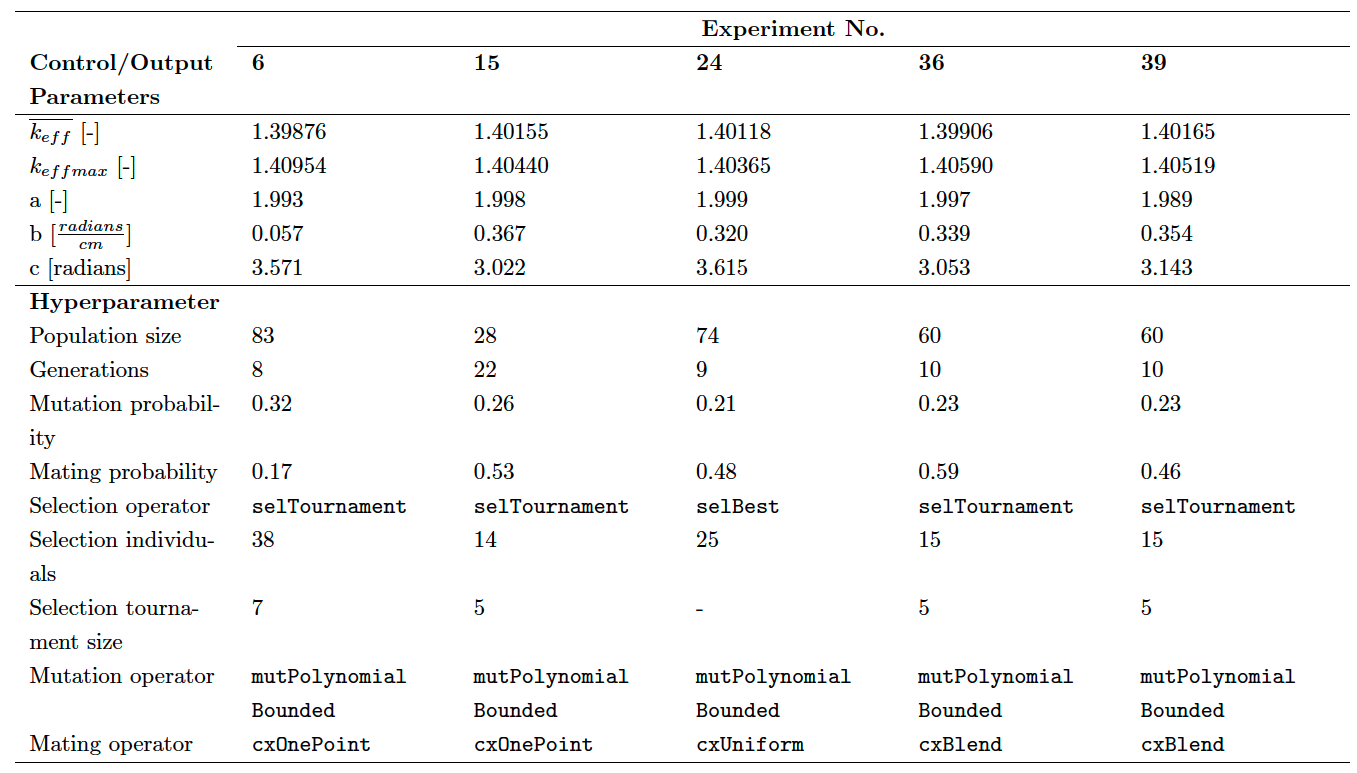
\includegraphics[width=0.85\linewidth]{figures/rollo-demo-best.png} 
    \end{table}
\end{frame}

\begin{frame}
    \frametitle{Completed Stage 2-2: Results from best hyperparameter set}
    \begin{figure}[]
        \centering
        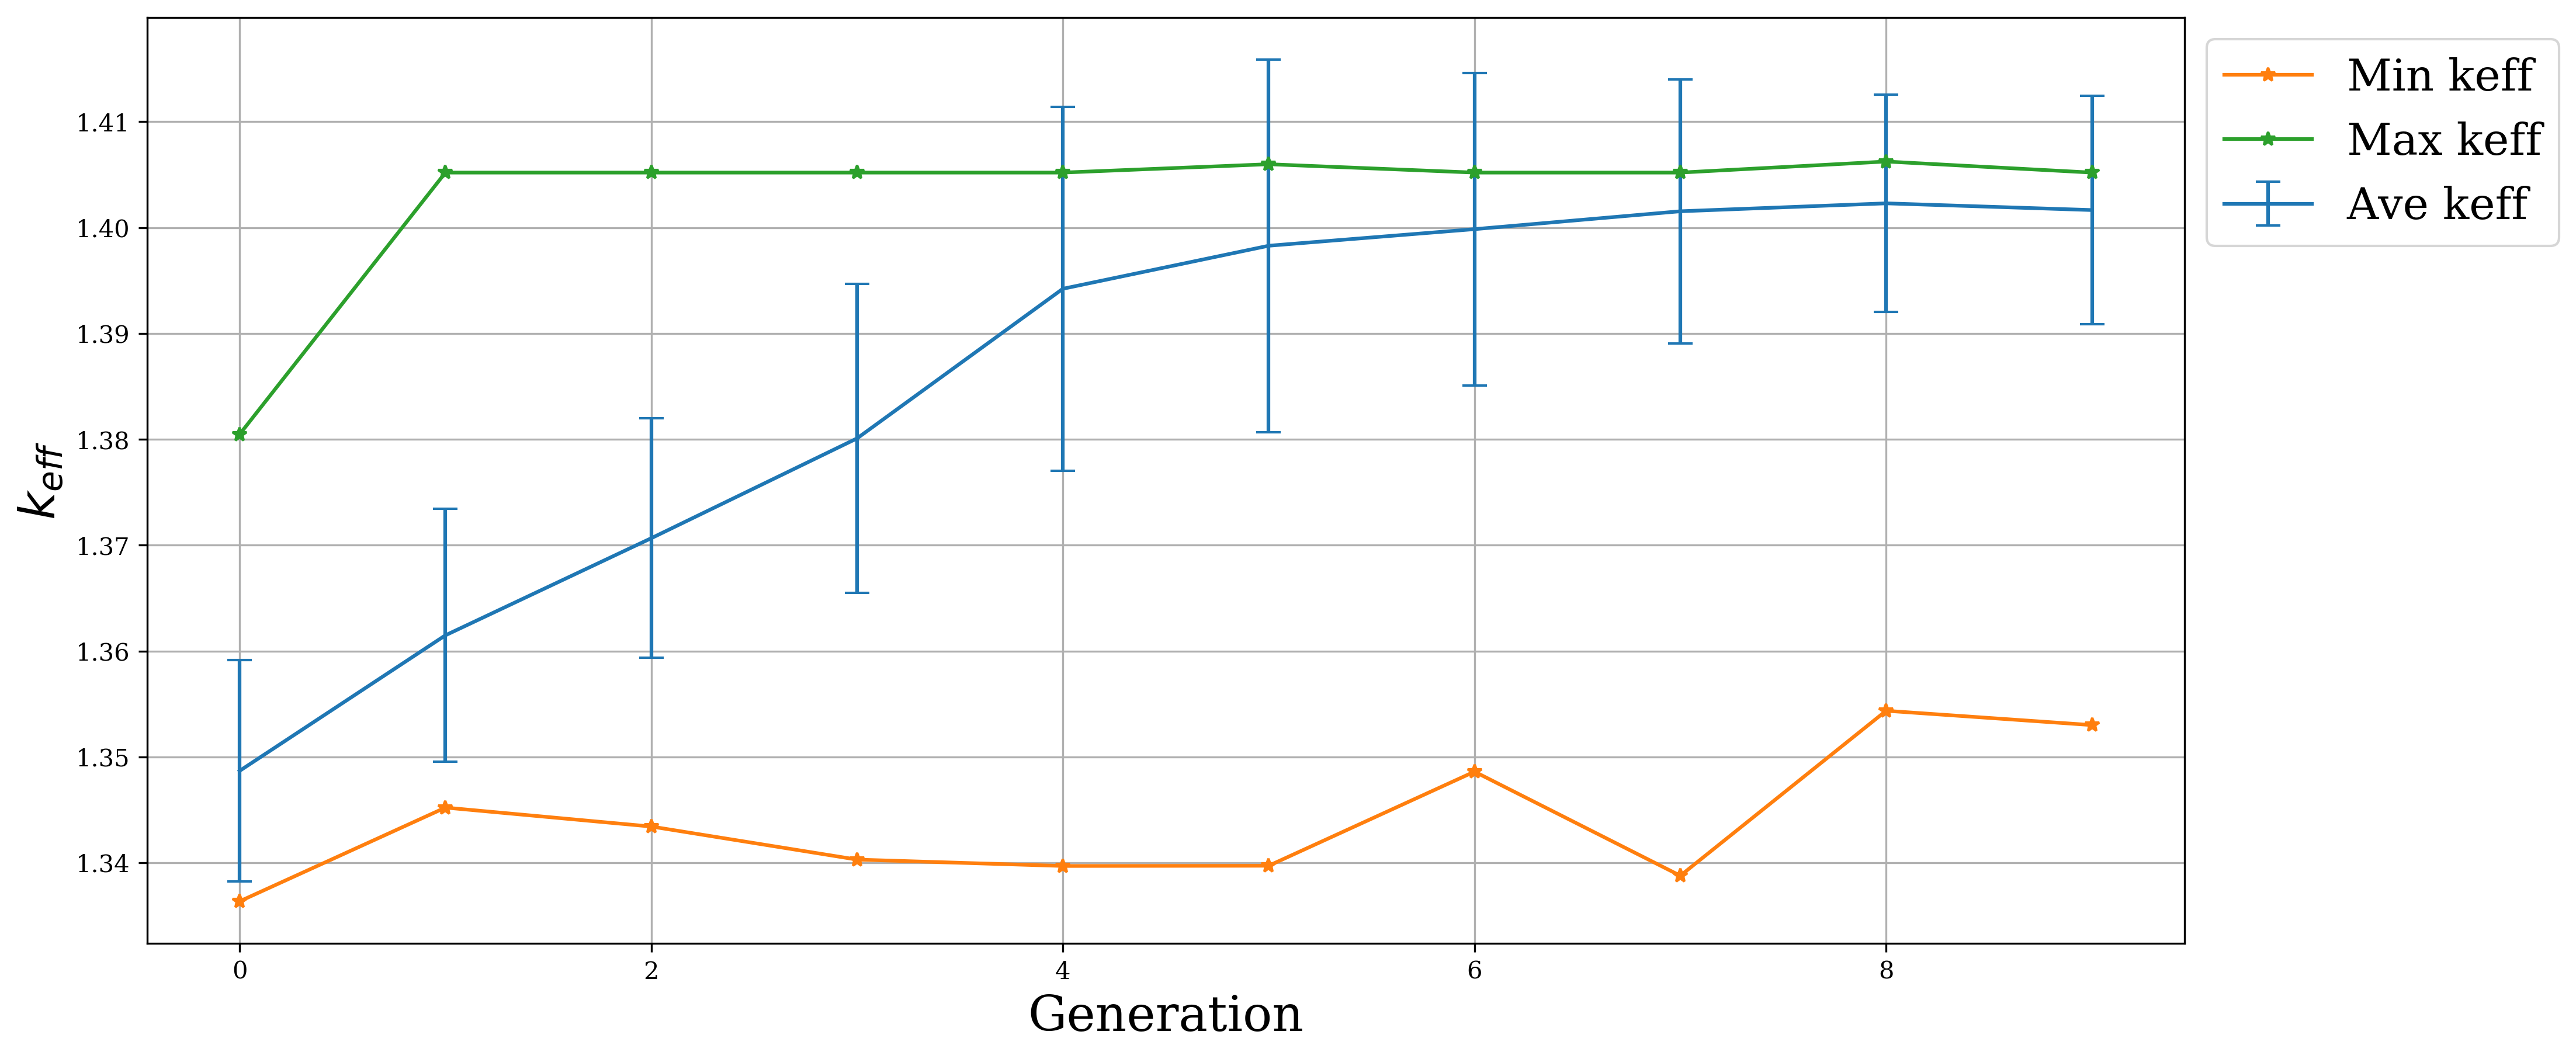
\includegraphics[width=\linewidth]{../docs/figures/keff_conv_39.png}
        \caption{39$^{th}$ Experiment's $k_{eff}$ evolution.}
    \end{figure}
\end{frame}

\begin{frame}
    \frametitle{Completed Stage 2-2: Results from best hyperparameter set}
    TRISO particle packing fraction peaks in the center 
    of the slab, showing that if the optimization problem focuses purely on the 
    slab's neutronics by maximizing $k_{eff}$, the fuel tends to culminate in the 
    middle. 

    \begin{figure}[]
        \centering
        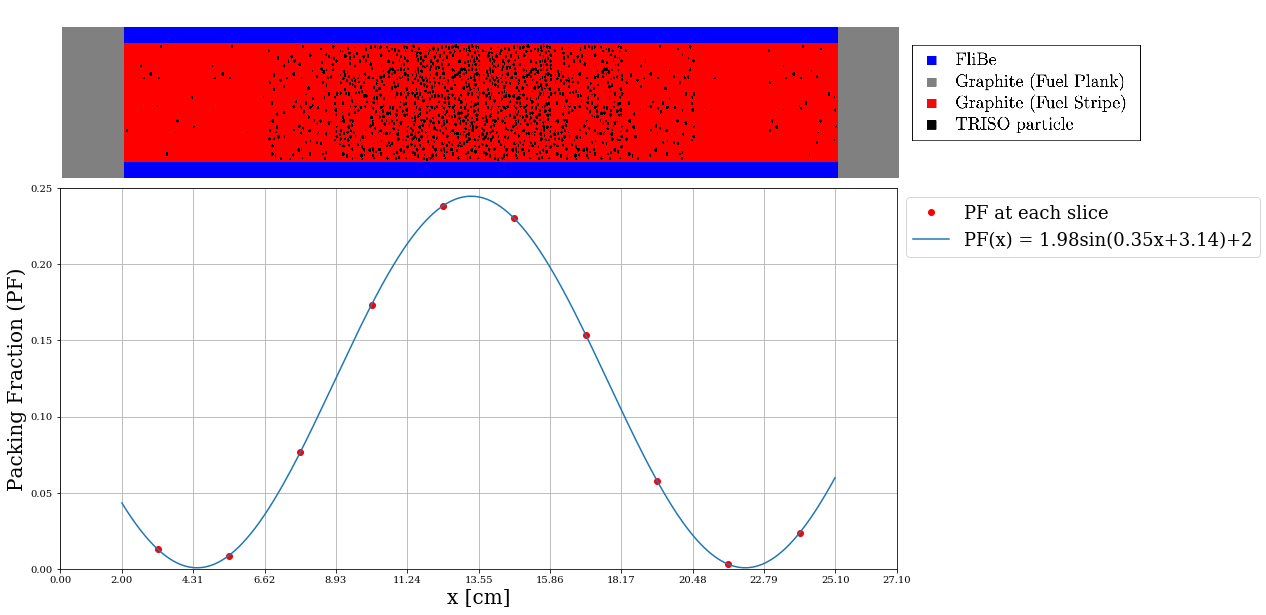
\includegraphics[width=0.8\linewidth]{../docs/figures/triso_distribution_sine_39.png} 
        \caption{Experiment 39 packing distribution that produced 
        $k_{eff max} = 1.40519 \pm 0.00130$. 
        $PF(x) = (1.98\ sin(0.35x+3.14)+2)  \times NF$ sine distribution. }
        \label{fig:triso_distribution_sine_39}
    \end{figure}
\end{frame}